\documentclass[UTF8]{ctexart}
\usepackage{ctex}
\usepackage{geometry}
\usepackage{enumitem}
\usepackage{indentfirst}
\usepackage{color}
\usepackage{fancyhdr}
\usepackage{amsmath}
\usepackage{graphicx}
\usepackage{amssymb}
\usepackage{tikz}
\usepackage{cases}
\usepackage{array}
\usepackage{pgfplots}
\usepackage{tkz-euclide}
\usepackage{mathrsfs}
% 设置纸张和页边距——A4
\geometry{papersize={21cm,29.7cm}}
\geometry{left=3.18cm,right=3.18cm,top=2.54cm,bottom=2.54cm}

% 一级标题靠左
\CTEXsetup[format={\Large\bfseries}]{section}

% 去除页眉
\pagestyle{plain}

%设置段间距
\addtolength{\parskip}{.4em}
%%设置行间距
%\usepackage{setspace}
%\setstretch{2.5}

% 开始文档内容
\begin{document}

\title{信号与系统课程笔记:Lecture 23:S域系统分析的剩余问题}
\author{授课教师:秦雨潇 \\
        笔记记录:曹时成}
\date{2023 年 11 月 29 日(第十三周,周三)}
\maketitle

\section{系统框图/模拟图}
\subsection{三个基本逻辑单元}
\begin{figure}[h]
    \raggedright   %使图片靠左放置
    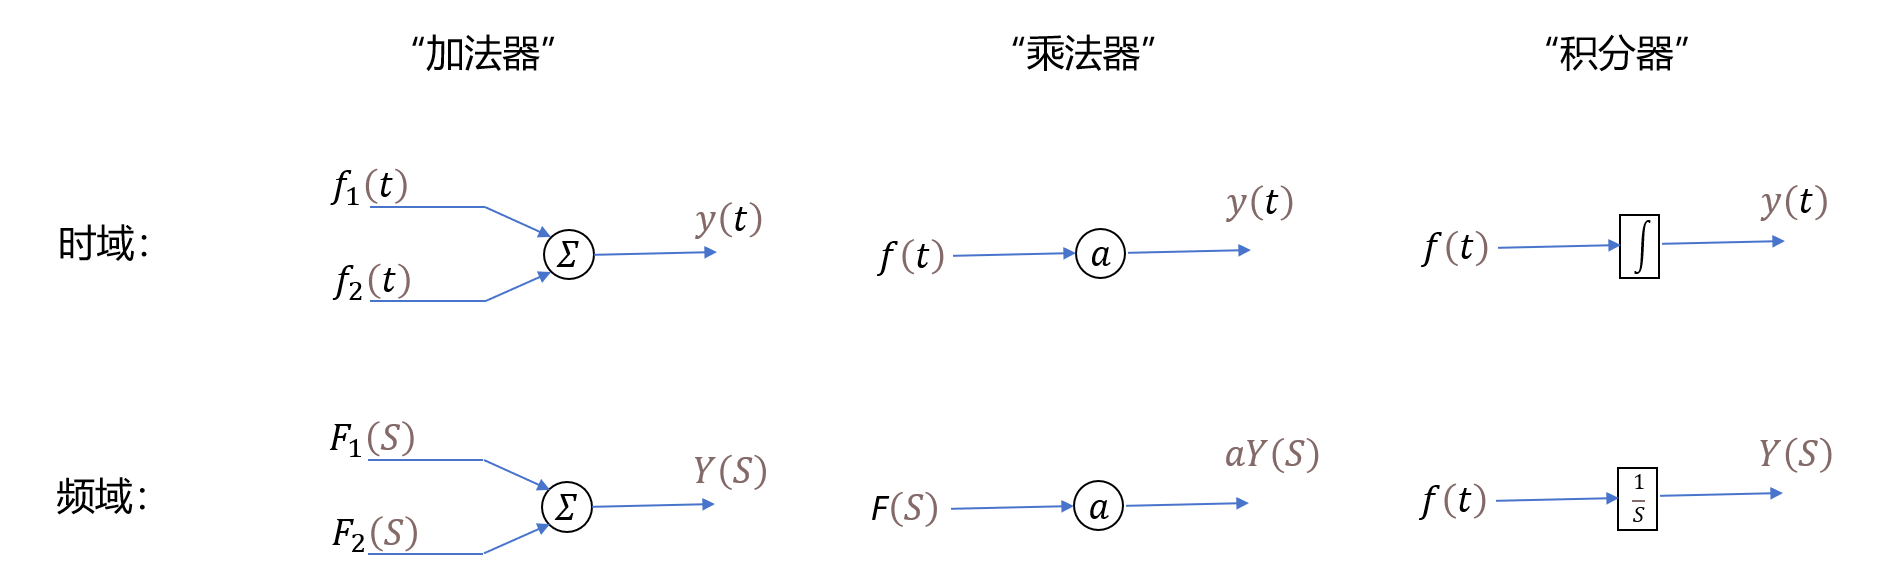
\includegraphics[scale=0.25]{1.png}
\end{figure}
\subsection{时域框图}
(1)$y''(t) + ay'(t) + by(t) = cf(t)$ \par
要点1:$y''(t)\longrightarrow \boxed{\text{$\int $}}\longrightarrow y'(t)\longrightarrow \boxed{\text{$\int $}}\longrightarrow y(t)$ \par
于是原式可写为:$f(t) +(-a)y'(t) + (-b)y(t)=y''(t)$ \par
\begin{figure}[h]
    \centering         %使图片居中放置
    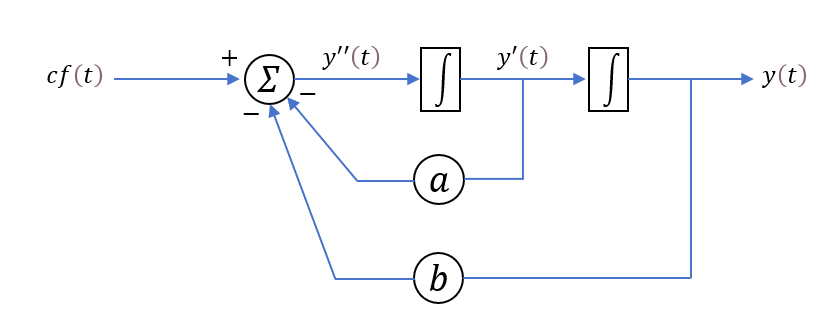
\includegraphics[scale=0.60]{2.png}
\end{figure}
\qquad  \par

(2)$y''(t) + ay'(t) + by(t) = cf(t)+df'(t)$ \par
$\because $ 考虑系统是LTI系统  \par
$\therefore  $ $df(t)\longrightarrow dy(t)$ \par
\quad   $df'(t)\longrightarrow dy'(t)$ \par
\begin{figure}[h]
    \centering         %使图片居中放置
    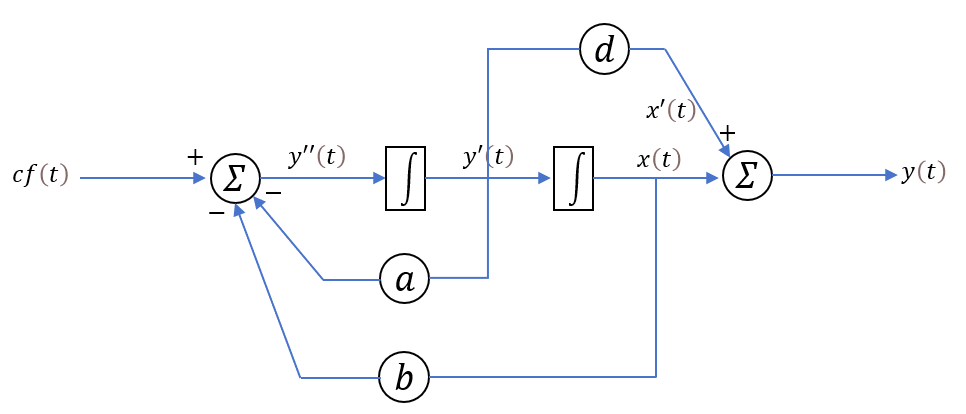
\includegraphics[scale=0.55]{3.png}
\end{figure}
(3)$y''(t) + ay'(t) + by(t) = cf(t)+df'(t)+ef''(t)$ \par
\begin{figure}[h]
    \centering         %使图片居中放置
    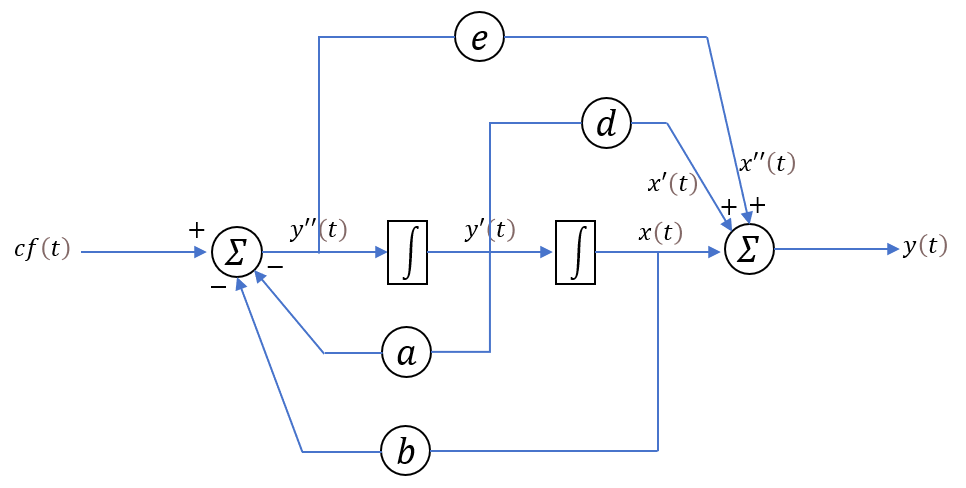
\includegraphics[scale=0.55]{4.png}
\end{figure}
\subsection{S域框图}
第一种: f(t)换成F(s),与y(t)换成Y(s),加法和乘法不变,积分变成$\boxed{\text{$\frac{1}{s}  $}}$ \par
第二种: $Y(s)=H(s)F(s)=F(s)\frac{cs+d}{(s+a)(s+b)}=F(s)\cdot \frac{k_1}{s+a} \cdot \frac{k_2}{s+b} $ \par
“串联形式”:\par
\begin{figure}[h]
    \raggedright   % 使图片靠左放置
    \hspace{2em}   % 在左侧添加 1em 的水平空白
    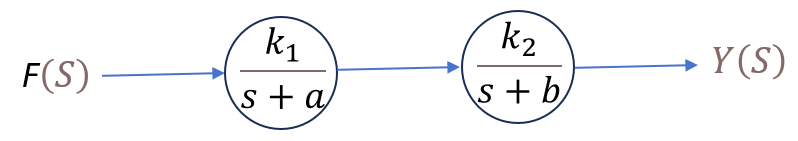
\includegraphics[scale=0.25]{5.png}
\end{figure}
第三种: $Y(s)=F(s)(\frac{z_1}{s+p_1} +\frac{z_2}{s+p_2} )$ \par
“并联形式”:
\begin{figure}[h]
    \raggedright   % 使图片靠左放置
    \hspace{2em}   % 在左侧添加 1em 的水平空白
    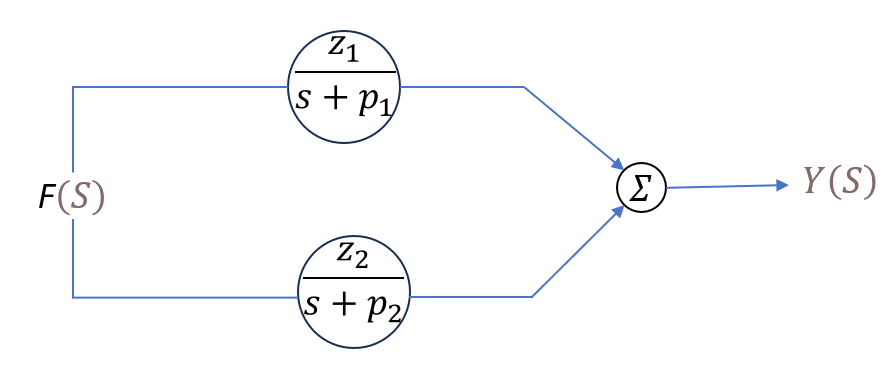
\includegraphics[scale=0.25]{6.png}
\end{figure}

\section{系统流图}
Graph \par
顶点:vertex \par
边:edge(有向/无向) \par
(3)$y''(t) + ay'(t) + by(t) = cf(t)+df'(t)+ef''(t)$ \par
\begin{figure}[h]
    \centering         %使图片居中放置
    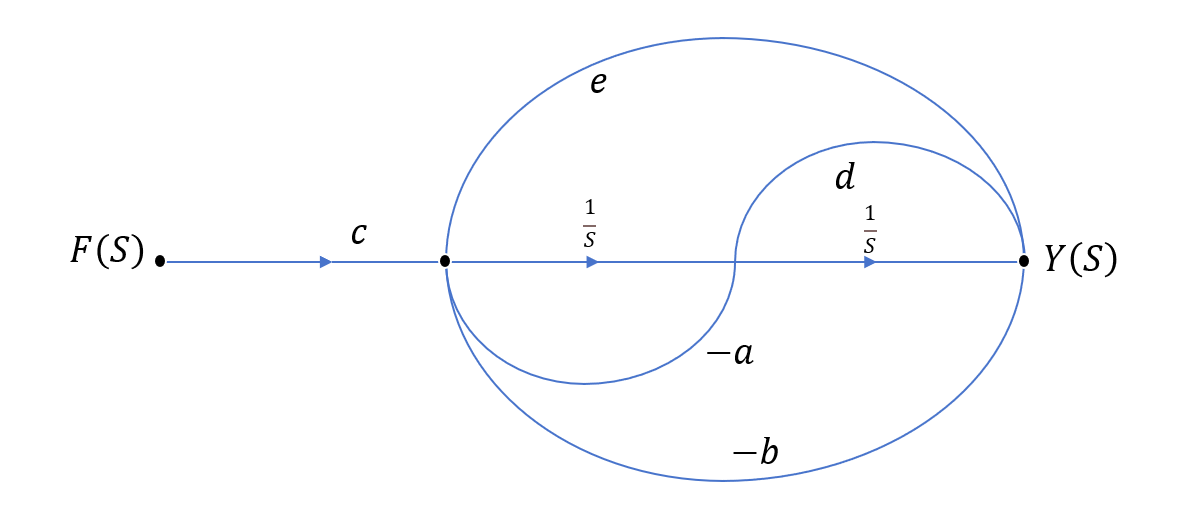
\includegraphics[scale=0.5]{7.png}
\end{figure}
\section{梅森公式}
计算系统流图的H(s)\par
课后自行看书理解!\par

\section{电路的复频域的表达形式(书上第5章第2节)}
(1)电容\par
时域:\par
\qquad $i(t)=c\frac{du(t)}{dt},u(t)=\frac{1}{c}\int_{0}^{t} i(t) \,dt +u(0_-)  $\par
S域:\par
\qquad $I(t)=csU(s)-cU(0_-),U(s)=\frac{1}{s} U(0_-)+\frac{1}{cs} I(s) $\par
S域电路:\par
\qquad \par
\begin{figure}[h]
    \centering         %使图片居中放置
    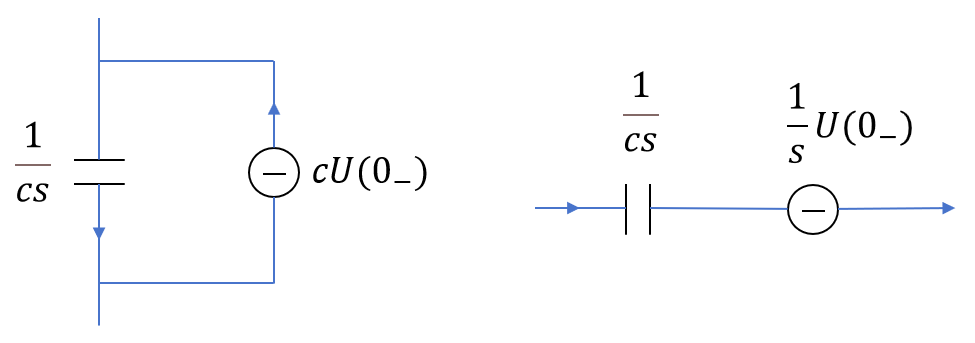
\includegraphics[scale=0.35]{8.png}
\end{figure}
“P”算子 \par
(2)电感\par
时域:\par
\qquad $u(t)=L\frac{d}{dt}i(t),i(t)=\frac{1}{L}\int_{0}^{t} u(\tau ) \,d\tau +i(0_-)   $\par
S域:\par
类比于电容的S域自己写出\par
S域电路:“串联”,“并联”\par
基尔霍夫定律依然适用\par

\section{系统稳定性的判定}
\subsection{从定义出发}
\qquad $\int_{\mathbb{R} } |h(t) \vert  \,dt <+\infty $\par
\subsection{零极图中的极点}
(1)无重根情况下:$H(s)=\sum_{i = 1}^{N} \frac{z_i}{s-p_i}\longleftrightarrow z_ie^{-p_it}=h(t)  $\par
有几点在jw轴右边则表明系统不稳定\par
(2)结论:教科书6.2.2节表6.1 \qquad 12个例子\par
$\textcircled{1} $ \; 所有极点都在jw轴以左:稳定 \par
$\textcircled{2} $ \; 只要有一个极点在jw轴右或双极点在jw轴上:不稳定 \par
$\textcircled{3} $ \; 单极点在jw轴上:临界稳定 \par
\qquad 临界稳定:h(t)=u(t),稳不稳定取决于输入 \par
\subsection{劳斯准则}
\qquad $a_ns^n+a_{n-1}s^{n-1}+a_{n-2}s^{n-2}+\cdots +a_{1}s+a_0=0$\par
\end{document}